\documentclass[11pt,a4paper]{article}

\usepackage{fullpage}
\usepackage{hyperref}
\usepackage{graphicx}
\usepackage{subcaption}
\usepackage{array}
\usepackage{cite}
\usepackage{float}

\usepackage{fancyhdr}
\pagestyle{fancy}
\fancyhf{}
\usepackage{todonotes}                %% notes from the authors

\renewcommand{\headrulewidth}{0pt}
\renewcommand{\footrulewidth}{0pt}

\newcommand\Tstrut{\rule{0pt}{2.6ex}}       % "top" strut
\newcommand\Bstrut{\rule[-0.9ex]{0pt}{0pt}} % "bottom" strut
\newcommand{\TBstrut}{\Tstrut\Bstrut} % top&bottom struts
\newcommand*{\escape}[1]{\texttt{\textbackslash#1}}

\fancypagestyle{firstpagefooter} {
	\lfoot{\tiny{Version: 25.09.2018}}
	\cfoot{}
	\rfoot{\thepage}
	
}

\lfoot{Name: Nicolas K\"uchler Legi: 14-712-129}
\rfoot{\thepage}

\begin{document}

\title{Advanced Systems Lab Report\\ \normalsize{Autumn Semester 2018}}
\author{Name: Nicolas K\"uchler\\Legi: 14-712-129}
\date{
	\vspace{4cm}
	\textbf{Grading} \\
	\vspace{0.5cm}
	\begin{tabular}{|c|c|}
		\hline  \textbf{Section} & \textbf{Points} \\
		\hline  1                &                 \\ 
		\hline  2                &                 \\ 
		\hline  3                &                 \\ 
		\hline  4                &                 \\ 
		\hline  5                &                 \\ 
		\hline  6                &                 \\ 
		\hline  7                &                 \\ 
		\hline \hline Total      &                 \\
		\hline 
	\end{tabular} 
}
\maketitle
\thispagestyle{firstpagefooter}

\newpage

\section{System Overview (75 pts)}
\todo{check 20-35 pages}
Describe the implementation of your system and highlight design decisions relevant for the experiments. Explain how messages are parsed and how statistics are gathered in a multi-threaded setting. Provide figures containing all the threads and queues in your system (including the network and the memcached servers). Include illustrations that show how requests of different types are handled (e.g., components involved in processing the request and method calls). Please include all details necessary to understand artifacts and effects in your experiments that arise from your implementation choices. \todo{remove}


The system is a middleware platform for the popular main-memory key-value store \emph{memcached}. \todo{cite memcached.org}
It enables to balance the read workload between up to three memcached instances possibly located on different servers by replicating all writes to all memcached instances.


\subsection{Middleware Architecture}
\subsubsection{High-Level Overview}

\begin{figure}
	\centering
	\includegraphics[width=\linewidth]{data/system-overview.png}
	\caption{System Overview}
\end{figure}
\todo{do properly with pdf and number components to reference them}

On start up of the middleware a configured number of worker-threads and a single net-thread are started.
Each worker-thread builds a tcp connection to each memcached server which is kept open during the run of the middleware.


The net-thread \emph{(NetThread.java)} listens on a configured tcp port for client requests. The different client channels are handled using a Selector.
After decoding the incoming request in the net-thread (see \ref{request-decoding}) they are put into a queue.

The worker-threads \emph{(WorkerThread.java)} take requests from the queue and process them according to their their type. (see \ref{request-processing}). Then they send back the response to the client via the channel.

\subsubsection{Request}
The middleware supports set, get and multi-get requests.

Logically each request from a client is represented using an instance of \emph{SetRequest.java}, \emph{GetRequest.java} or \emph{MultiGetRequest.java}. They all inherit basic functionality from \emph{AbstractRequest.java}.
These request objects are created in the net-thread by the decoder (see \ref{request-decoding}) and put into a \emph{BlockingQueue} where they wait to be processed by a worker-thread (see \ref{request-processing}).

Apart from containing the request command, they also serve as a container for the tcp socket channel to the client and for timestamps collected at different points in the system (see \ref{measured-points}).
\todo{write about that they contain server id}

\subsubsection{Request Decoding}\label{request-decoding}
In the net-thread the incoming requests are decoded one by one using the function \emph{decode(ByteBuffer buffer)} of the request decoder \emph{(RequestDecoder.java)}.
Since every request needs to pass this function the decoding is done on byte level to avoid unnecessary overhead.
Apart from checking that the client request is supported by the middleware the decoder also verifies that the request is completely read. In case the decoder encounters an unsupported operation or a malformed request \emph{(UnknownRequest.java)}, the request is discarded until a newline character is read. Then an error is returned to the client and a log entry is created. If a request is not complete yet, the decoder signals the net-thread that more is expected and the net-thread will append the next content arriving from the client channel to the same buffer to complete the request.

In the following the decoding of the three different request types is explained. \todo{maybe add decoding state machine}

\paragraph{SET} \texttt{set <key> <flags> <exptime> <bytes>[noreply]\textbackslash r\textbackslash n<datablock>\textbackslash r\textbackslash n} 

After reading the set in the beginning of the command, the decoder skips over key, flags and expiration time before reading the bytes field to determine if the data block is complete. If the request is complete, a \emph{SetRequest.java} is created.

\paragraph{GET / MULTI-GET} \texttt{get <key>\textbackslash r\textbackslash n} or \texttt{get <key1> <key2> ... <key10>\textbackslash r\textbackslash n}

After reading the get in the beginning of the command, the decoder determines the number of keys and checks that the request is complete. If there is only a single key, then a \emph{GetRequest.java} is created. Otherwise a \emph{MultiGetRequest.java} is created.

For get and multi-get requests the decoder assigns each request a server (or for sharded mutli-get multiple servers) in a round-robin scheme. (see more on workload balancing in \ref{workload-balancing})


\subsubsection{Request Processing}\label{request-processing}

A worker-thread takes a request from the queue and processes it depending on the request type.

\emph{ServerMessage.java} by calling the \emph{getServerMessages()} function of the request object.

The worker-thread sends these messages one after the other to the specified servers.
The different channels to the servers are monitored using a Selector. Whenever a response of a server arrives it 
is given to the request using the function \emph{putServerResponse(serverId, buffer)}. The request assembles all responses and when all arrived a response is written back to the client through the socket channel.

\paragraph{Set} The request command is sent to all servers. If all servers answer with \texttt{STORED\textbackslash r\textbackslash n} then \texttt{STORED\textbackslash r\textbackslash n} is sent to the client. 

If at least one server answers with an error message, then the error message which arrived last is relayed to the client.

\paragraph{Get} The request command is sent to the server specified by the round-robin scheme in the net-thread.
The response of the server is directly relayed to the client.

\paragraph{MultiGet} The processing is different depending on the sharded/non-sharded mode. In case of non-sharded mode, the processing is identical to a get request where the message is sent to one server and the response is directly relayed to the client. In case of sharded mode, the request is split into up to three smaller requests\todo{explain splitting rule} . Each of them is sent to the server determined by the round-robin scheme. Then each server response is fed back to the request that is responsible for reordering the results. When all responses arrived, the reordered response is sent to the client.

\subsubsection{Workload Balancing}\label{workload-balancing}
The round robin scheme applied for get and multi-get requests allows to balance the read-workload among multiple servers.

As described in \ref{request-decoding} each get and multi-get request becomes the server ids allocated in the net-thread.
For get and multi-get requests in non-sharded mode this is only one server id. For multi-get requests in sharded mode this is a set of server ids. (if the number of keys is larger than the number of server then this will be all servers).

Since the net-thread is a singleton and the request queue offers first come first served processing of requests, the order in which they are processed does not change and hence when neglecting network related effects it can be expected that the work will be distributed evenly among the available servers.

Another form of work balancing takes place with the different number of worker threads. For a single worker-thread there is no balancing. \todo{continue this argument}

The balancing of the read workload comes at the cost of the write-workload. Since the value in each set request is replicated in all memcached servers, the server service time is determined by the slowest server. 


\subsubsection{Logging Infrastructure}

log4j2 asynchronous loggers

\todo{cite: https://logging.apache.org/log4j/2.x/manual/async.html}

\subsection{Experimental Setup}

\subsubsection{Measured Points}\label{measured-points}
\paragraph{Client}
The memtier clients provide average set/get throughput and response time.

\paragraph{Middleware}

In the middleware the arrival of the request, the time the request is put into the queue, the time a request is taken from the queue, the time a message has been sent to the server, the time of the server response and the time the request left the middleware are recorded.

This allows to calculate response time, net-thread processing time, queue waiting time, worker-thread processing time and individual server service time per request type.

In addition the throughput in the five second window is recorded.


In addition in the net-thread the number of arrivals in five seconds window is recorded
The length of the queue is sampled every 5 seconds.

\begin{figure}
	\centering
	\includegraphics[width=0.8\linewidth]{data/response-time-decomposition.png}
	\caption{components of client response time}
\end{figure}
\todo{do properly with pdf and color scheme}

\subsubsection{Statistic}

Each worker-thread has a separate statistic unit \emph{(Statistic.java)} which is updated after the processing of each request with the method \emph{update(request)}.  
The statistic unit is collecting online average and sample standard deviation of several metrics over a five second window using \emph{Welford's Algorithm}.\cite{Knuth:1997:ACP:270146}

\begin{equation}
	\bar{x}_n = \bar{x}_{n-1} + \frac{x_n -\bar{x}_{n-1}}{n}
\end{equation}

\begin{equation}
	M_{2,n} = M_{2,n-1} + (x_n - \bar{x}_{n-1})(x_n - \bar{x}_n)
\end{equation}

\begin{equation}
	s^2_n = \frac{M_{2,n}}{n-1}
\end{equation}

Every five seconds each worker logs these metrics to a log file.




\subsubsection{Base Configuration}
- memcached (version) 1 thread
- 4096B values
- memtier benchmark (version) with configuration
\subsubsection{Simulation}\label{simulation}
- simulated on azure cloud using up to three client, two middleware and three server virtual machines (vm) (give specs of VM's)
- before every experiment the bandwidth between all involved virtual machines is measured using iperf \todo{cite}. This in combination with the 4096B values results in an estimate for the maximal achievable throughput for the given vm configuration and helps to identify when the network bandwidth is the bottleneck of the system.
- baseline without middleware run separately all other experiments were run without shutting down the vm to allow comparison of results not only within an experiment but also between experiments.
- after 10 sec warm up and cooldown phase ensured stable 1 minute throughput performance by checking coefficient of variation
- before every run, restart all memcached instances, initialize them by filling all keys, restart mw's


\todo{System Overview
(Mapping code to functionality / Explanation how queues and threads are implemented 15)
insert overview picture}

- Description of the data-structures for holding connections 6 

- Parsing Requests: 
(Description how requests are parsed 6)
\todo{insert processing schematic}

- Processing of Requests in Worker:
- Set Request
- Get Request
- MultiGet Request (Sharded vs Non Sharded)
Description how SET requests are processed 6 Description how GET requests are processed 6 Description how Multi-GET requests are processed 6 

- Description how work is balanced (if not round-robin: proof required) 15 
-> here get, multiget sharded, maybe also worker balances work

- Statistics (Explanations related to statistics 15)
-> Sampling of queue size, arrival rate in 5 sec windows
-> Welfords Algorithm Online Averages with Std Deviation within 5 sec windows, reported 5sec aggregations (allows insight std dev gives insight in window without slowing down system too much through logging)
\todo{cite welford algorithm}


\section{Baseline without Middleware (75 pts)}

In this section the performance characteristics of the memtier clients and memcached servers in the azure cloud are studied.

\subsection{One Server}

%Both, for a read-only and write-only workload plot the throughput and the response time as a function of NumClients. All clients are connected to a single memcached instance.

%Use 3 load generating VMs, with one memtier (CT=2) each, and vary the number of virtual clients (VC) per memtier thread between 1 and 32. Show how the behavior of the server changes as we add more clients.

This experiment analyses the behaviour of the system with 3 load generating VM's and a single server VM. The detailed experiment configuration is presented in the table below.

For every configuration the throughput and response time as measured on the client is used.

Every graph contains the sample standard deviation over the 3 repetitions as an error metric.
To validate the measurements the interactive law with a client thinking time Z of 0 is shown in every throughput and response time graph.

As mentioned in section \ref{simulation} before running the experiment the network bandwidth between the VM's was tested using \emph{iperf}. From these measurements a maximal achievable throughput was derived by considering the value size of 4096B. This bandwidth limit is also shown in the throughput graphs.


\begin{center}
	\scriptsize{
		\begin{tabular}{|l|c|}
			\hline Number of servers                & 1                        \\ 
			\hline Number of client machines        & 3                        \\ 
			\hline Instances of memtier per machine & 1                        \\ 
			\hline Threads per memtier instance     & 2                        \\
			\hline Virtual clients per thread       & [1, 2, 4, 8, 12, 16, 24, 32]\\ 
			\hline Workload                         & Write-only and Read-only \\
			%\hline Multi-Get behavior               & N/A                      \\
			%\hline Multi-Get size                   & N/A                      \\
			%\hline Number of middlewares            & N/A                      \\
			%\hline Worker threads per middleware    & N/A                      \\
			\hline Repetitions                      & 3 (at least 1 minute each)\\ 
			\hline 
		\end{tabular}
	}
\end{center}


\begin{figure}
	\begin{subfigure}[b]{.49\linewidth}
		\centering
		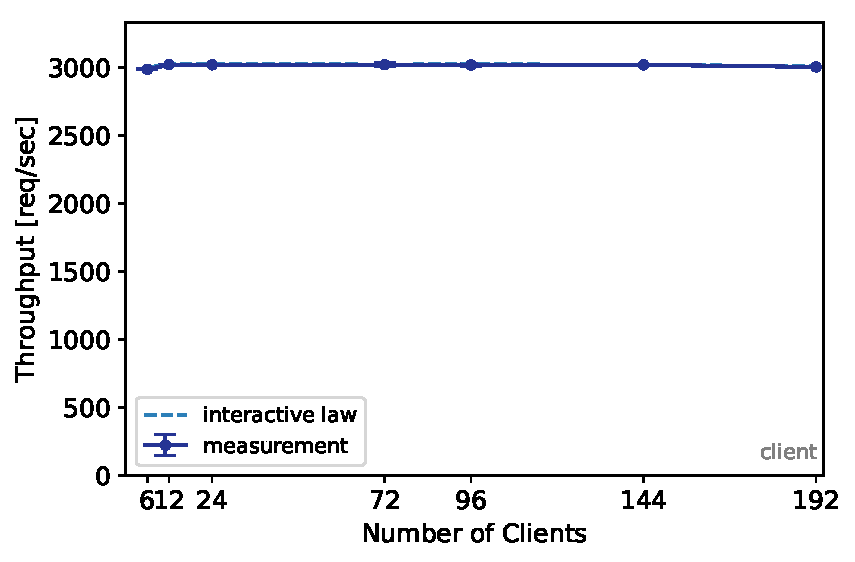
\includegraphics[width=\linewidth]{data/exp21_ro_tp_nc.pdf}
	\end{subfigure}\hfill
	\begin{subfigure}[b]{.49\linewidth}
		\centering
		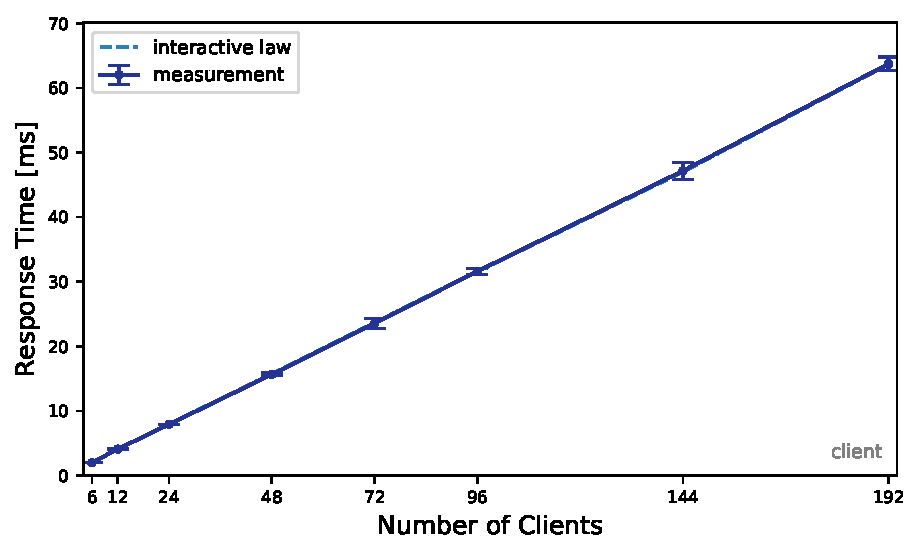
\includegraphics[width=\linewidth]{data/exp21_ro_rt_nc.pdf}
	\end{subfigure}%
	\caption{Throughput and response time with interactive law in read-only workload with one memcached server.}
	\label{exp21_ro_nc}
\end{figure}


\begin{figure}
	\begin{subfigure}[b]{.49\linewidth}
		\centering
		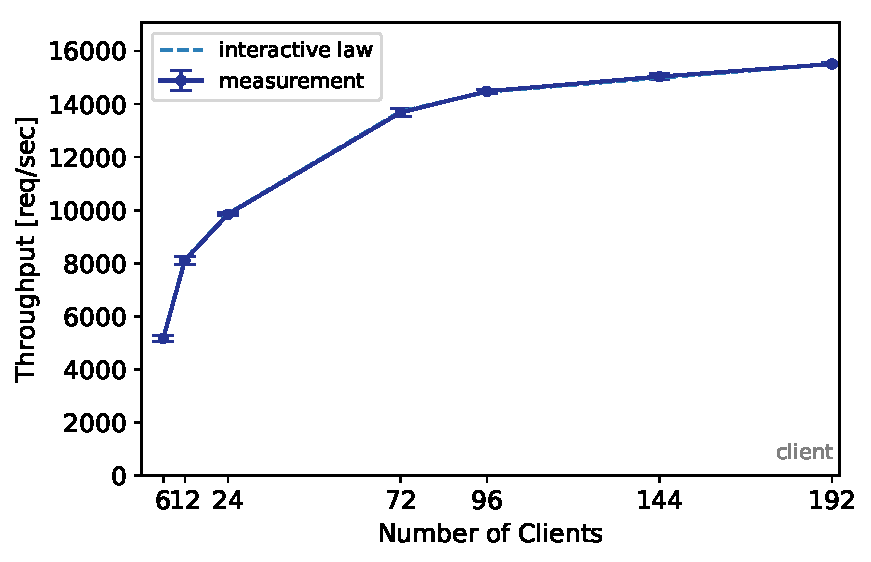
\includegraphics[width=\linewidth]{data/exp21_wo_tp_nc.pdf}
	\end{subfigure}\hfill
	\begin{subfigure}[b]{.49\linewidth}
		\centering
		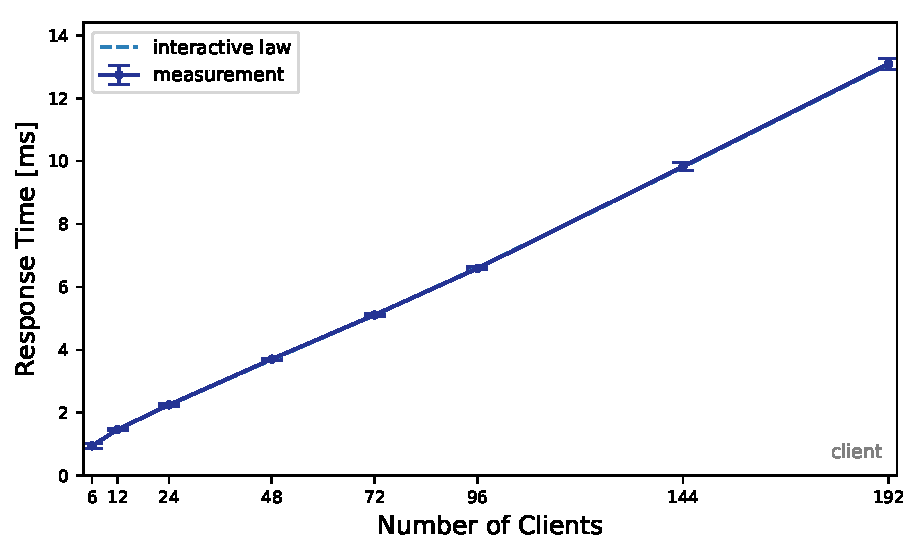
\includegraphics[width=\linewidth]{data/exp21_wo_rt_nc.pdf}
	\end{subfigure}%
	\caption{Throughput and response time with interactive law in write-only workload with one memcached server.}
	\label{exp21_wo_nc}
\end{figure}



\subsubsection{Explanation}

%Describe in which phase the memcached servers are under-saturated, saturated, or over-saturated. Describe how throughput and response time correlate. Explain what further conclusions can be drawn from the experiment.

As shown in figure \ref{exp21_ro_nc}, the throughput saturation for the read-only workload is already reached at 6 clients because the upload bandwidth of the single server VM limits the throughput. Before the experiment, the server VM upload bandwidth was measured to be 99.6 MBit/sec. When using a value size of 4096B, this results in a maximum possible throughput of 3040 ops/sec for a read-only workload because all the values need to be sent from the server VM to one of the 3 client VM's. 

Consequently increasing the number of clients has almost no effect on the throughput while the response time grows linearly because more clients results in more requests on the server that wait to be sent to a client VM. \todo{maybe be more precice about why linear increase: I think more clients => more requests => every request needs to "wait" a bit longer on server vm}

In figure \ref{exp21_wo_nc} it can be observed that for a write-only workload the throughput saturation is reached at 72 clients. In this experiment the bottleneck is not the bandwidth but rather the memcached server. 
As expected the throughput first increases in the number of clients while the memcached servers are still under-saturated and then the response 


\subsection{Two Servers}

%For a read-only and write-only workload plot throughput and response time as a function of NumClients. The clients are connected to two memcached instances. 

%Use 1 load generating VM, with one memtier (CT=1) connected to each memcached instance (two memcache instances in total), and vary the number of virtual clients (VC) per memtier thread between 1 and 32. Show how the behavior of the server changes and explain what conclusions we can draw from this experiment.

\begin{center}
	\scriptsize{
		\begin{tabular}{|l|c|}
			\hline Number of servers                & 2                        \\ 
			\hline Number of client machines        & 1                        \\ 
			\hline Instances of memtier per machine & 2                        \\ 
			\hline Threads per memtier instance     & 1                        \\
			\hline Virtual clients per thread       & [1, 2, 4, 8, 12, 16, 24, 32]\\ 
			\hline Workload                         & Write-only and Read-only \\
			%\hline Multi-Get behavior               & N/A                      \\
			%\hline Multi-Get size                   & N/A                      \\
			%\hline Number of middlewares            & N/A                      \\
			%\hline Worker threads per middleware    & N/A                      \\
			\hline Repetitions                      & 3 (at least 1 minute each) \\ 
			\hline 
		\end{tabular}
	} 
\end{center}



\begin{figure}
	\begin{subfigure}[b]{.49\linewidth}
		\centering
		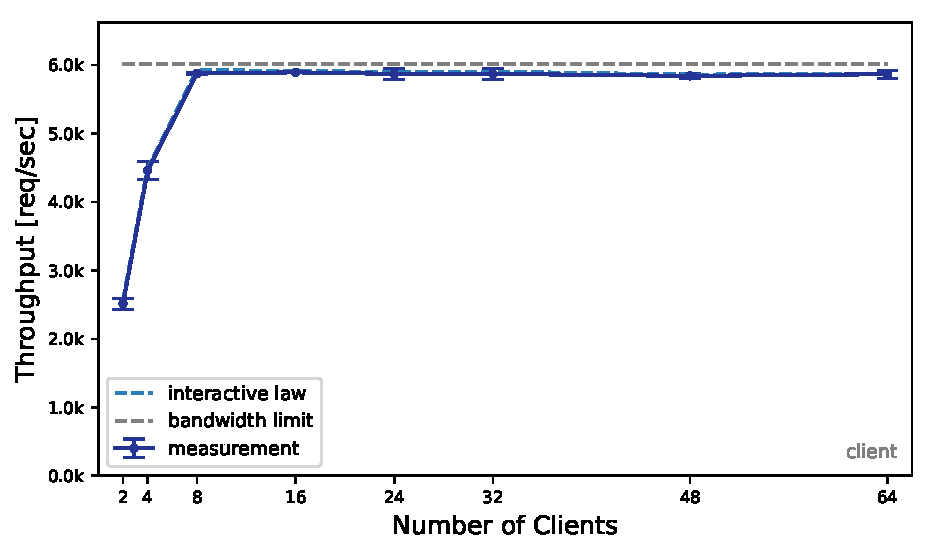
\includegraphics[width=\linewidth]{data/exp22_ro_tp_nc.pdf}
	\end{subfigure}\hfill
	\begin{subfigure}[b]{.49\linewidth}
		\centering
		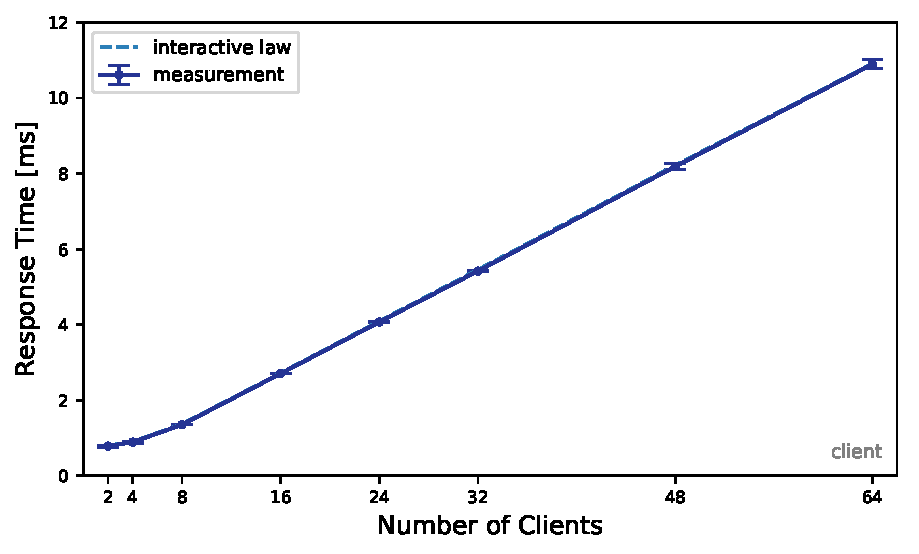
\includegraphics[width=\linewidth]{data/exp22_ro_rt_nc.pdf}
	\end{subfigure}%
	\caption{Throughput and response time with interactive law in read-only workload with one load generating VM.}
	\label{exp22_ro_nc}
\end{figure}




\begin{figure}
	\begin{subfigure}[b]{.49\linewidth}
		\centering
		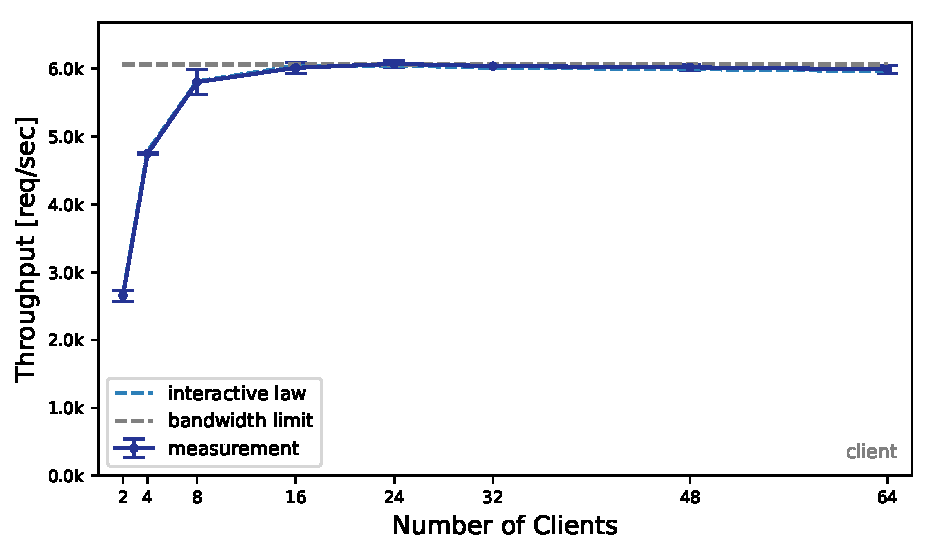
\includegraphics[width=\linewidth]{data/exp22_wo_tp_nc.pdf}
	\end{subfigure}\hfill
	\begin{subfigure}[b]{.49\linewidth}
		\centering
		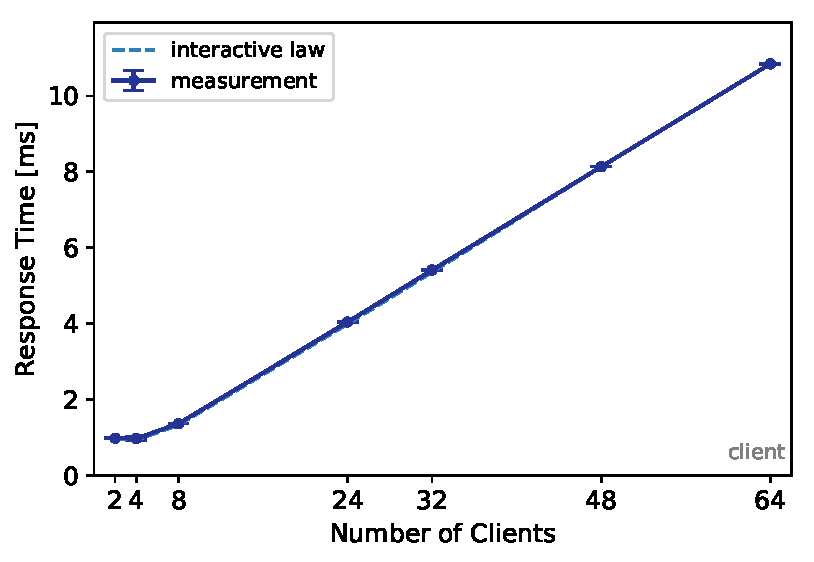
\includegraphics[width=\linewidth]{data/exp22_wo_rt_nc.pdf}
	\end{subfigure}%
	\caption{Throughput and response time with interactive law in write-only workload with one load generating VM.}
	\label{exp22_wo_nc}
\end{figure}



\subsubsection{Explanation}

%Describe how this experiment compares to the previous section. Which results are the same and which ones differ? Explain what further conclusions can be drawn from the experiment.

For a read-only workload the throughput saturation is reached at 8 clients, as shown in figure \ref{exp22_ro_nc}, because the upload bandwidth of the two servers limits the possible throughput. The measured total upload bandwidth between the 2 server VM's and the client VM is 199 MBit/sec which results in an estimate of 6062 ops/sec for the maximally achievable throughput when using values of 4096B. Before the saturation point is reached at 8 clients, increasing the number of clients results in a higher throughput as expected because the system is still under-saturated. \todo{maybe mention that because cutoff is so abruptly that it could be expected that with 8 clients memcached itself is not saturated at all}

Using a write-only workload with values of 4096B the situation is similar but here instead of the upload bandwidth of the server VM's the bottleneck is the upload bandwidth of the load generating client VM. The measured 199 MBit/sec total upload bandwidth of the client VM limits the throughput of the system to 6062 ops/sec. So as a consequence  the throughput saturation is reached at \todo{choose either 8 or 16} clients as shown in figure \ref{exp22_wo_nc}.


\subsection{Summary}


\begin{center}
	{Maximum throughput of different VMs.}
	\begin{tabular}{|l|p{2cm}|p{2cm}|p{4cm}|}
		\hline                        & Read-only workload & Write-only workload & Configuration gives max. throughput \\ 
		\hline One memcached server   & 2962 ops/sec       & 14097 ops/sec & 6 clients for read-only 72 clients for write-only\\ 
		\hline One load generating VM & 5878 ops/sec       &  5802 or 6012 ops/sec & 8 clients for read-only 8/16 clients for write-only\\ 
		\hline 
	\end{tabular}
\end{center}


%Write at least two paragraphs about how both results relate. Describe what is the bottleneck of this setup is. If the maximum throughput for both experiments is the same, explain why. If it is not the case, explain why not. Write down key take-away messages about the behaviour of the memtier clients and the memcached servers.

\paragraph{Comparison of one memcached server vs. one load generating VM}
For a read-only workload both experiments are bound by the network upload bandwidth of the server VM(s).
Despite the fact that they are both network bound, they have a different maximum throughput because having an additional server in the second experiment gives two times the upload bandwidth between server and client VMs and thus resulting in approximately two times the throughput.

The different throughput for write-only workload is explained by considering that only the second experiment is bound by the network. Namely by the upload bandwidth of the client VM. The bottleneck in the first experiment is memcached which saturates for around 72 clients.

\paragraph{Comparison of workloads}
In the first experiment with one memcached server the throughput is different between write and read workload. This is because in a read-only workload the server needs to transport the value and some control structure which is more than 4096B. For write-only the server VM only needs to transmit the 8 byte confirmation message \texttt{STORED\textbackslash r\textbackslash n} to the client VM. 

Despite the fact that in the second experiment with only one load generating VM the throughput for read-only and write-only is almost identical the bottleneck is a different part of the system. For read-only it is the upload bandwidth of the two server VMs and for the write-only workload it is the upload bandwidth of the load generating client VM.

\paragraph{Key take-away messages}
\begin{itemize}
	\item a single server VM cannot handle more than 3000 ops/sec in a read-only workload
	\item a single client VM cannot simulate a higher write-only workload than 6000 ops/sec
	\item in a write-only workload the point of saturation for a single memcached server is around 14000 ops/sec
\end{itemize}


\section{Baseline with Middleware (90 pts)}

In this set of experiments, you will have to use 1 load generator VM and 1 memcached server, measuring how the throughput of the system changes when increasing the number of clients. Scaling virtual clients inside memtier has to be done as explained in the previous sections. Plot both throughput and response time as measured on the middleware.

\subsection{One Middleware}

Connect one load generator machine (one instance of memtier with CT=2) to a single middleware and use 1 memcached server. Run a read-only and a write-only workload with increasing number of clients (between 2 and 64) and measure response time \emph{both at the client and at the middleware}, and plot the throughput and response time measured in the middleware.

Repeat this experiment for different number of worker threads inside the middleware: 8, 16, 32, 64.

\begin{center}
	\scriptsize{
		\begin{tabular}{|l|c|}
			\hline Number of servers                & 1                        \\ 
			\hline Number of client machines        & 3                        \\ 
			\hline Instances of memtier per machine & 1                        \\ 
			\hline Threads per memtier instance     & 2                        \\
			\hline Virtual clients per thread       & [1..32]                  \\ 
			\hline Workload                         & Write-only and Read-only \\
			\hline Multi-Get behavior               & N/A                      \\
			\hline Multi-Get size                   & N/A                      \\
			\hline Number of middlewares            & 1                        \\
			\hline Worker threads per middleware    & [8..64]                  \\
			\hline Repetitions                      & 3 or more (at least 1 minute each)                \\ 
			\hline 
		\end{tabular}
	} 
\end{center}

\todo{need better reference to the experiment}

\begin{figure}
	\begin{subfigure}[b]{.49\linewidth}
		\centering
		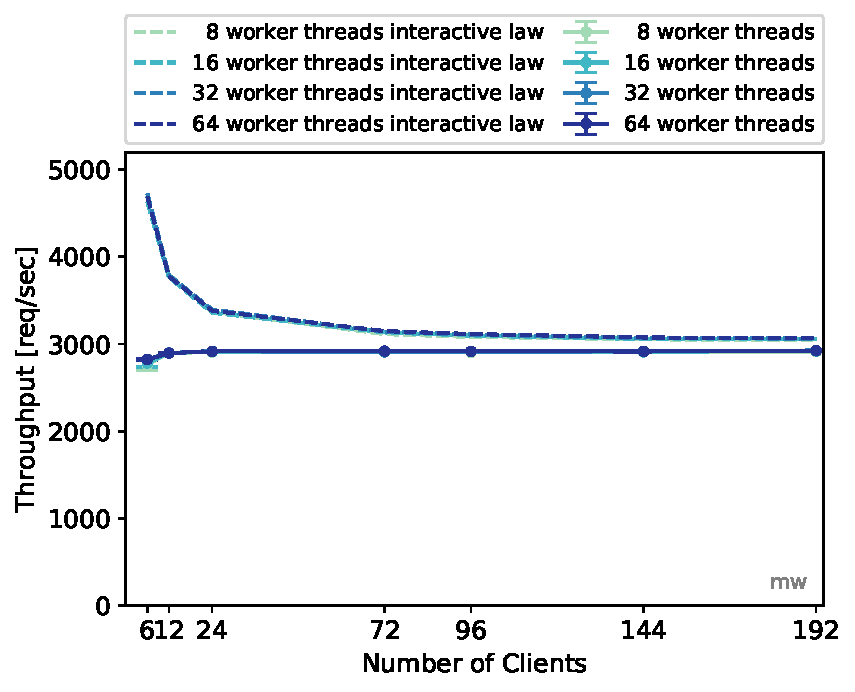
\includegraphics[width=\linewidth]{data/exp31_ro_tp_nc_w.pdf}
		%\caption{Throughput}\label{fig1a}
	\end{subfigure}\hfill
	\begin{subfigure}[b]{.49\linewidth}
		\centering
		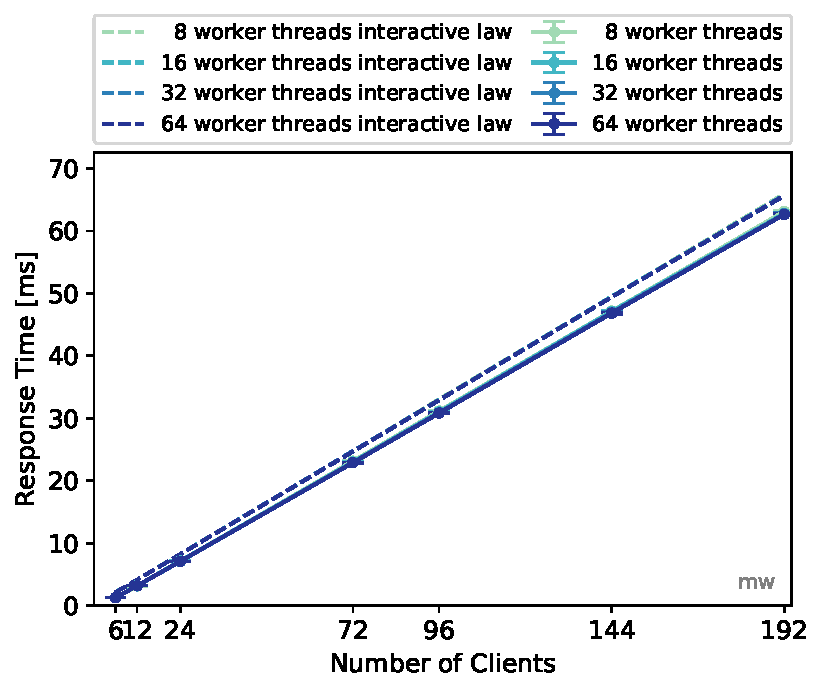
\includegraphics[width=\linewidth]{data/exp31_ro_rt_nc_w.pdf}
		%\caption{Response Time}\label{fig1b}
	\end{subfigure}%
	\caption{Throughput and response time with interactive law in read-only workload}
\end{figure}

\begin{figure}
	\begin{subfigure}[b]{.49\linewidth}
		\centering
		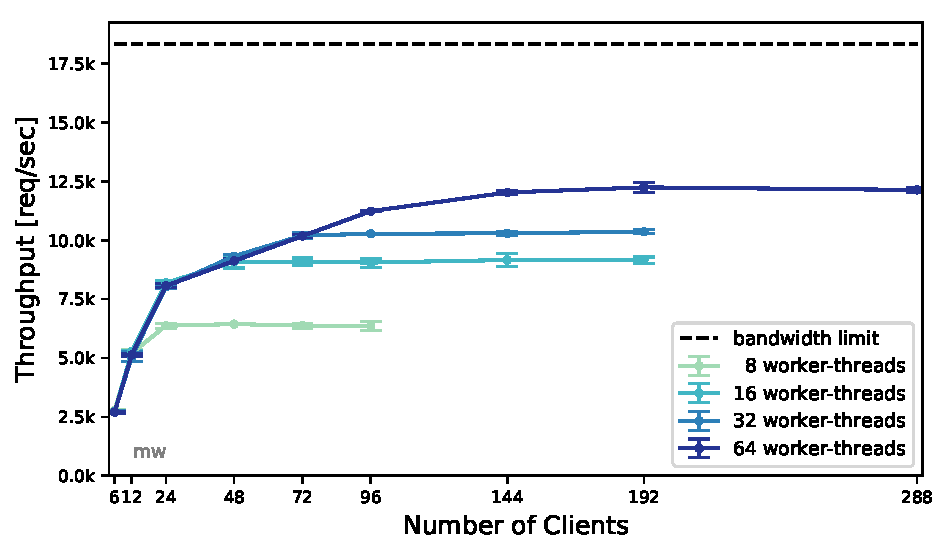
\includegraphics[width=\linewidth]{data/exp31_wo_tp_nc_w.pdf}
		%\caption{Throughput}\label{fig1a}
	\end{subfigure}\hfill
	\begin{subfigure}[b]{.49\linewidth}
		\centering
		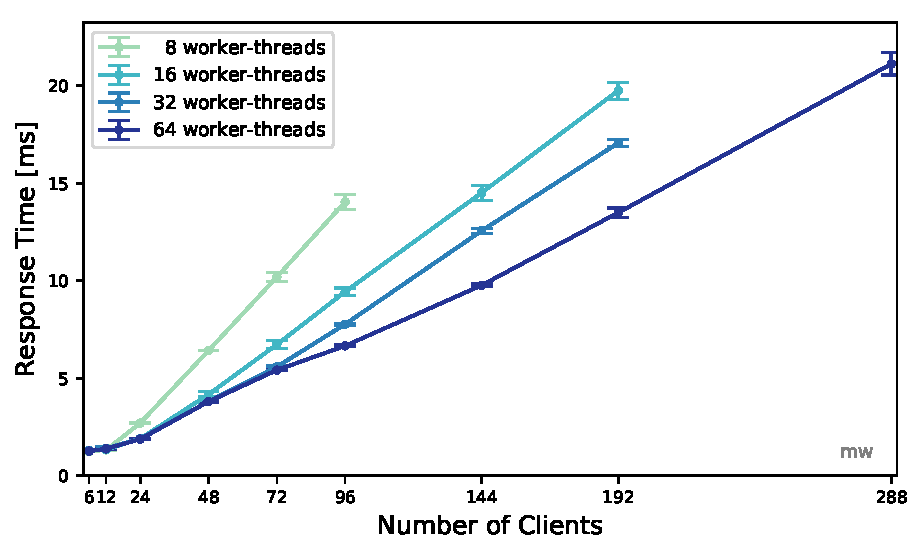
\includegraphics[width=\linewidth]{data/exp31_wo_rt_nc_w.pdf}
		%\caption{Response Time}\label{fig1b}
	\end{subfigure}%
	\caption{Throughput and response time with interactive law in write-only workload}
\end{figure}

\subsubsection{Explanation}

Provide a detailed analysis of the results (e.g., bottleneck analysis, component utilizations, average queue lengths, system saturation). Add any additional figures and experiments that help you illustrate your point and support your claims.

\subsection{Two Middlewares}

Connect one load generator machine (two instances of memtier with CT=1) to two middlewares and use 1 memcached server. Run a read-only and a write-only workload with increasing number of clients (between 2 and 64) and measure response time \emph{both at the client and at the middleware}, and plot the throughput and response time as measured in the middleware.

Repeat this experiment for different number of worker threads inside the middleware: 8, 16, 32, 64.

If in your experiment the middleware is not the bottleneck, repeat the experiment that reaches the highest throughput but using two load generator VMs (each with 2x memtier CT=1) instead of one. Otherwise, explain how you know that the middlewares are the limiting factor in terms of throughput.

\begin{center}
	\scriptsize{
		\begin{tabular}{|l|c|}
			\hline Number of servers                & 1                        \\ 
			\hline Number of client machines        & 3                        \\ 
			\hline Instances of memtier per machine & 2                        \\ 
			\hline Threads per memtier instance     & 1                        \\
			\hline Virtual clients per thread       & [1..32]                  \\ 
			\hline Workload                         & Write-only and Read-only \\
			\hline Multi-Get behavior               & N/A                      \\
			\hline Multi-Get size                   & N/A                      \\
			\hline Number of middlewares            & 2                        \\
			\hline Worker threads per middleware    & [8..64]                  \\
			\hline Repetitions                      & 3 or more (at least 1 minute each)                \\ 
			\hline 
		\end{tabular}
	} 
\end{center}
\todo{need better reference to the experiment}

\begin{figure}
	\begin{subfigure}[b]{.49\linewidth}
		\centering
		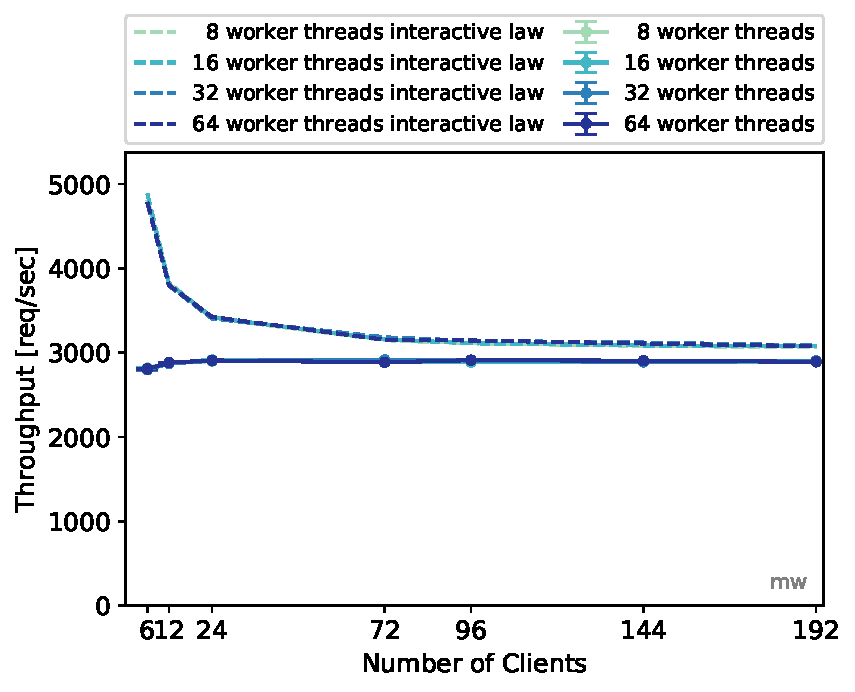
\includegraphics[width=\linewidth]{data/exp32_ro_tp_nc_w.pdf}
		%\caption{Throughput}\label{fig1a}
	\end{subfigure}\hfill
	\begin{subfigure}[b]{.49\linewidth}
		\centering
		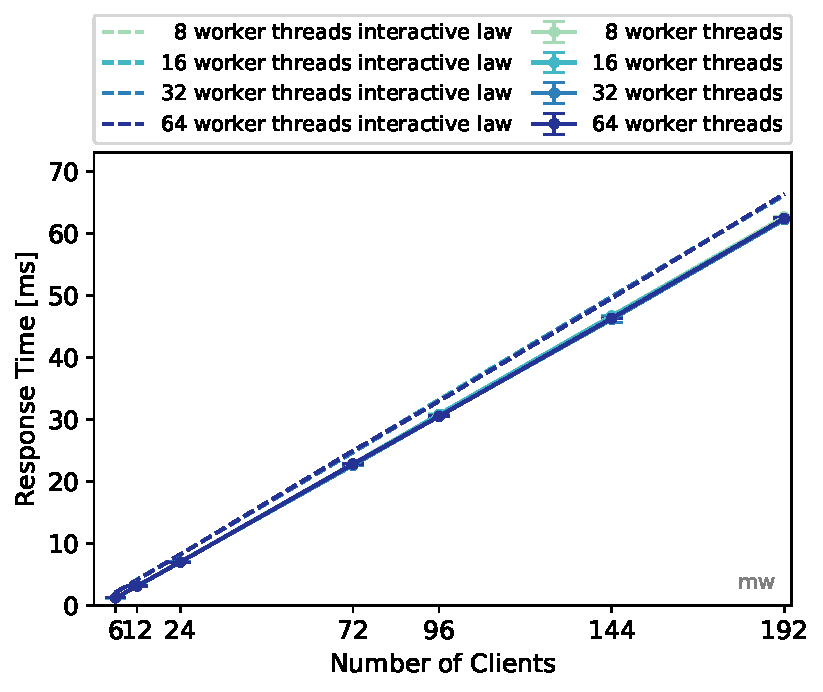
\includegraphics[width=\linewidth]{data/exp32_ro_rt_nc_w.pdf}
		%\caption{Response Time}\label{fig1b}
	\end{subfigure}%
	\caption{Throughput and response time with interactive law in read-only workload}
\end{figure}

\begin{figure}
	\begin{subfigure}[b]{.49\linewidth}
		\centering
		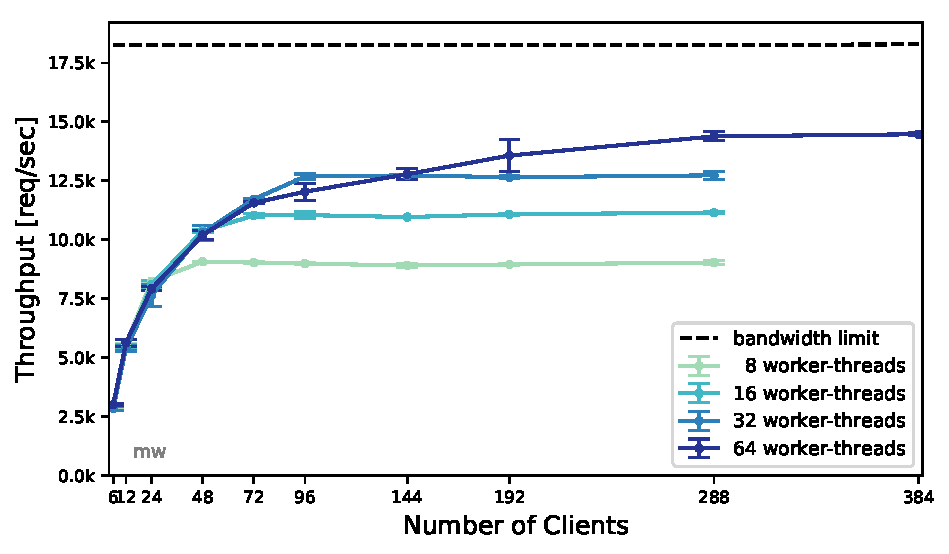
\includegraphics[width=\linewidth]{data/exp32_wo_tp_nc_w.pdf}
		%\caption{Throughput}\label{fig1a}
	\end{subfigure}\hfill
	\begin{subfigure}[b]{.49\linewidth}
		\centering
		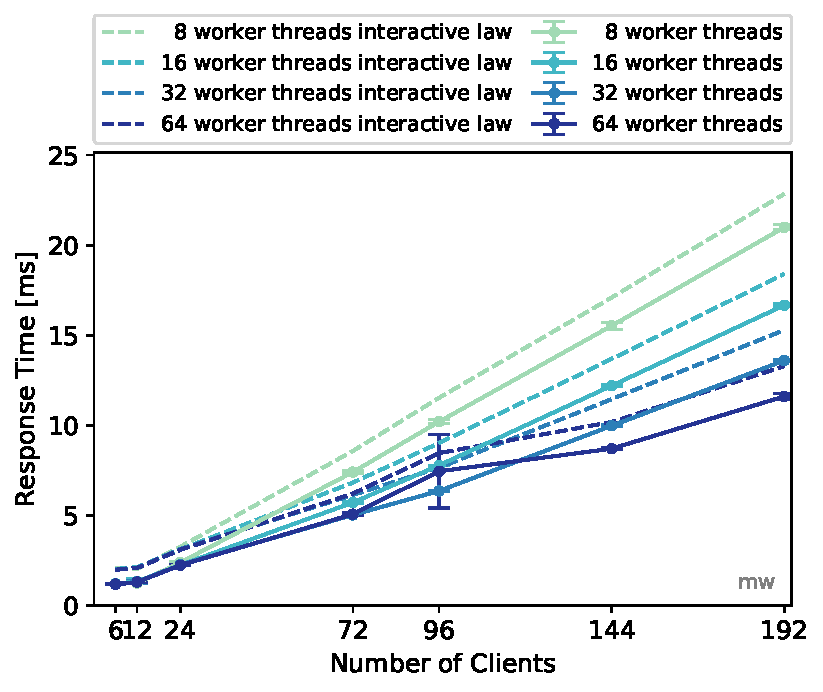
\includegraphics[width=\linewidth]{data/exp32_wo_rt_nc_w.pdf}
		%\caption{Response Time}\label{fig1b}
	\end{subfigure}%
	\caption{Throughput and response time with interactive law in write-only workload}
\end{figure}
\todo{reference back to baseline without mw here with 2 mw's and 64 worker threads basically reach in write-only the max}

\subsubsection{Explanation}

Provide a detailed analysis of the results (e.g., bottleneck analysis, component utilizations, average queue lengths, system saturation). Add any additional figures and experiments that help you illustrate your point and support your claims.

\subsection{Summary}

Based on the experiments above, fill out the following table. For both of them use the numbers from a single experiment to fill out all lines. Miss rate represents the percentage of GET requests that return no data. Time in the queue refers to the time spent in the queue between the net-thread and the worker threads.


\begin{center}
	{Maximum throughput for one middleware.}
	\begin{tabular}{|l|p{2cm}|p{2cm}|p{2cm}|p{2cm}|}
		\hline                                & Throughput & Response time & Average time in queue & Miss rate \\ 
		\hline Reads: Measured on middleware  &            &               &                       &           \\ 
		\hline Reads: Measured on clients     &            &               & n/a                   &           \\ 
		\hline Writes: Measured on middleware &            &               &                       & n/a       \\ 
		\hline Writes: Measured on clients    &            &               & n/a                   & n/a       \\ 
		\hline 
	\end{tabular}
\end{center}

\begin{center}
	{Maximum throughput for two middlewares.}
	\begin{tabular}{|l|p{2cm}|p{2cm}|p{2cm}|p{2cm}|}
		\hline                                & Throughput & Response time & Average time in queue & Miss rate \\ 
		\hline Reads: Measured on middleware  &            &               &                       &           \\ 
		\hline Reads: Measured on clients     &            &               & n/a                   &           \\ 
		\hline Writes: Measured on middleware &            &               &                       & n/a       \\ 
		\hline Writes: Measured on clients    &            &               & n/a                   & n/a       \\ 
		\hline 
	\end{tabular}
\end{center}

Based on the data provided in these tables, write at least two paragraphs summarizing your findings about the performance of the middleware in the baseline experiments.

\section{Throughput for Writes (90 pts)}

\subsection{Full System}

Connect three load generating VMs to two middlewares and three memchached servers. Run a write-only experiment. 
You need to plot throughput and response time measured on the middleware as a function of number of clients. The measurements have to be performed for 8, 16, 32 and 64 worker threads inside each middleware.

\begin{center}
	\scriptsize{
		\begin{tabular}{|l|c|}
			\hline Number of servers                & 3          \\ 
			\hline Number of client machines        & 3          \\ 
			\hline Instances of memtier per machine & 2          \\ 
			\hline Threads per memtier instance     & 1          \\
			\hline Virtual clients per thread       & [1..32]    \\ 
			\hline Workload                         & Write-only \\
			\hline Multi-Get behavior               & N/A        \\
			\hline Multi-Get size                   & N/A        \\
			\hline Number of middlewares            & 2          \\
			\hline Worker threads per middleware    & [8..64]    \\
			\hline Repetitions                      & 3 or more (at least 1 minute each)  \\ 
			\hline 
		\end{tabular}
	} 
\end{center}

\todo{need better reference to experiment}
\begin{figure}
	\begin{subfigure}[b]{.49\linewidth}
		\centering
		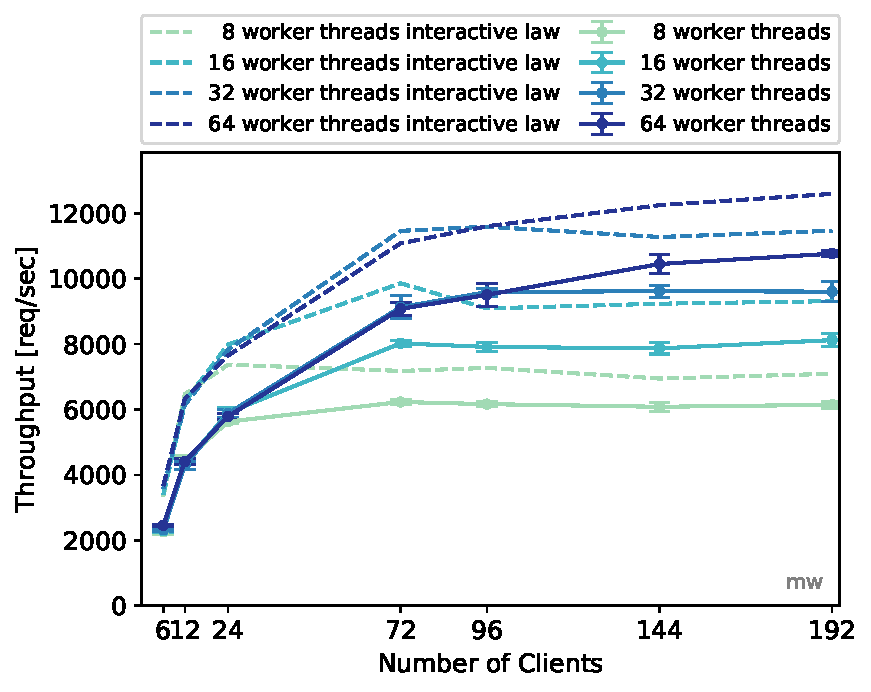
\includegraphics[width=\linewidth]{data/exp41_wo_tp_nc_w.pdf}
		%\caption{Throughput}\label{fig1a}
	\end{subfigure}\hfill
	\begin{subfigure}[b]{.49\linewidth}
		\centering
		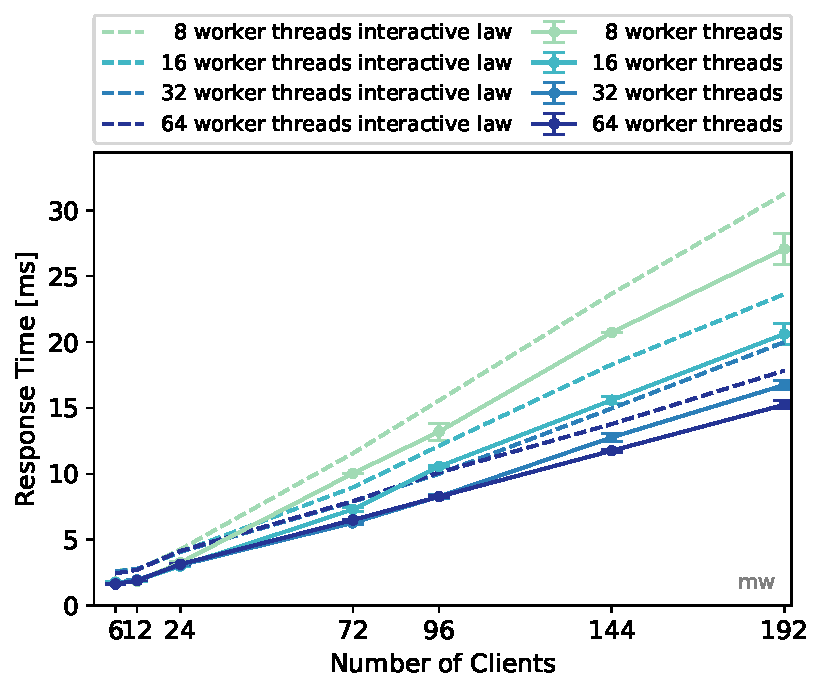
\includegraphics[width=\linewidth]{data/exp41_wo_rt_nc_w.pdf}
		%\caption{Response Time}\label{fig1b}
	\end{subfigure}%
	\caption{Throughput and response time with interactive law in write-only workload}
\end{figure}



\subsubsection{Explanation}

Provide a detailed analysis of the results (e.g., bottleneck analysis, component utilizations, average queue lengths, system saturation). Add any additional figures and experiments that help you illustrate your point and support your claims.

\subsection{Summary}

Based on the experiments above, fill out the following table with the data corresponding to the maximum throughput point for all four worker-thread scenarios.

\begin{center}
	{Maximum throughput for the full system}
	\begin{tabular}{|l|p{1.5cm}|p{1.5cm}|p{1.5cm}|p{1.5cm}|}
		\hline                                            & WT=8 & WT=16 & WT=32 & WT=64 \\ 
		\hline Throughput (Middleware)                    &      &       &       &       \\ 
		\hline Throughput (Derived from MW response time) &      &       &       &       \\ 
		\hline Throughput (Client)                        &      &       &       &       \\ 
		\hline Average time in queue                      &      &       &       &       \\ 
		\hline Average length of queue                    &      &       &       &       \\ 
		\hline Average time waiting for memcached         &      &       &       &       \\ 
		\hline 
	\end{tabular}
\end{center}

Based on the data provided in these tables, draw conclusions on the state of your system for a variable number of worker threads.

\section{Gets and Multi-gets (90 pts)}

For this set of experiments you will use three load generating machines, two middlewares and three memcached servers. Each memtier instance should have 2 virtual clients in total and the number of middleware worker threads is 64, or the one that provides the highest throughput in your system (whichever number of threads is smaller).

For multi-GET workloads, memtier will generate a mixture of SETs, GETs, and multi-GETs. Memtier only allows to specify the maximum number of keys in a multi-GET request. Therefore, be aware that requests can also contain fewer keys than the provided value. It is recommended to record the average size of the multi-GETs. You will have to measure response time on the client as a function of multi-get size, with and without sharding on the middlewares.
\todo{compare response time decomposition between sharded and non-sharded -> would expect sharded has longer wtt but shorter sst}

\subsection{Sharded Case}

Run multi-gets with 1, 3, 6 and 9 keys (memtier configuration) with sharding enabled (multi-gets are broken up into smaller multi-gets and spread across servers). Plot average response time as measured on the client, as well as the 25th, 50th, 75th, 90th and 99th percentiles.

\begin{center}
	\scriptsize{
		\begin{tabular}{|l|c|}
			\hline Number of servers                & 3                       \\ 
			\hline Number of client machines        & 3                       \\ 
			\hline Instances of memtier per machine & 2                       \\ 
			\hline Threads per memtier instance     & 1                       \\
			\hline Virtual clients per thread       & 2     		            \\ 
			\hline Workload                         & ratio=1:$<$Multi-Get size$>$             \\
			\hline Multi-Get behavior               & Sharded                 \\
			\hline Multi-Get size                   & [1..9]                  \\
			\hline Number of middlewares            & 2                       \\
			\hline Worker threads per middleware    & max. throughput config. \\
			\hline Repetitions                      & 3 or more (at least 1 minute each)               \\ 
			\hline 
		\end{tabular}
	} 
\end{center}

\todo{better reference to experiment}
\begin{figure}
	\begin{subfigure}[b]{.49\linewidth}
		\centering
		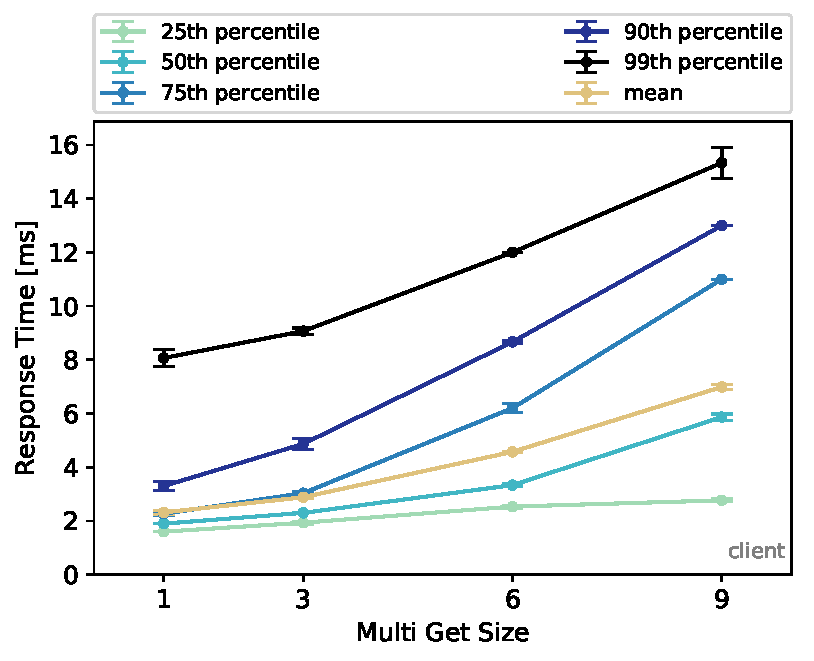
\includegraphics[width=\linewidth]{data/exp51_sharded_rt_mget_perc_client.pdf}
		%\caption{}\label{fig1a}
	\end{subfigure}\hfill
	\begin{subfigure}[b]{.49\linewidth}
		
	\end{subfigure}%
	\caption{Average response time and 25th, 50th, 75th, 90th and 99th percentiles of different multi-get sizes in sharded mode}
\end{figure}

\subsubsection{Explanation}

Provide a detailed analysis of the results (e.g., bottleneck analysis, component utilizations, average queue lengths, system saturation). Add any additional figures and experiments that help you illustrate your point and support your claims.

\subsection{Non-sharded Case}

Run multi-gets with 1, 3, 6 and 9 keys (memtier configuration) with sharding disabled. Plot average response time as measured on the client, as well as the 25th, 50th, 75th, 90th and 99th percentiles.

\begin{center}
	\scriptsize{
		\begin{tabular}{|l|c|}
			\hline Number of servers                & 3                       \\ 
			\hline Number of client machines        & 3                       \\ 
			\hline Instances of memtier per machine & 2                       \\ 
			\hline Threads per memtier instance     & 1                       \\
			\hline Virtual clients per thread       & 2                		 \\ 
			\hline Workload                         & ratio=1:$<$Multi-Get size$>$              \\
			\hline Multi-Get behavior               & Non-Sharded             \\
			\hline Multi-Get size                   & [1..9]                  \\
			\hline Number of middlewares            & 2                       \\
			\hline Worker threads per middleware    & max. throughput config. \\
			\hline Repetitions                      & 3 or more (at least 1 minute each)               \\ 
			\hline 
		\end{tabular}
	} 
\end{center}

\todo{better reference to experiment}
\begin{figure}
	\begin{subfigure}[b]{.49\linewidth}
		\centering
		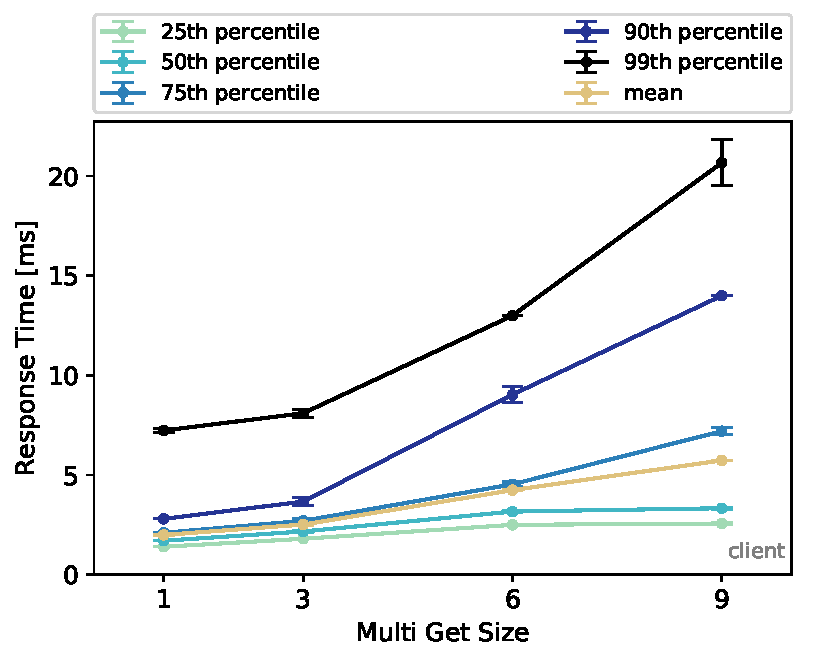
\includegraphics[width=\linewidth]{data/exp52_nonsharded_rt_mget_perc_client.pdf}
		%\caption{}\label{fig1a}
	\end{subfigure}\hfill
	\begin{subfigure}[b]{.49\linewidth}
		
	\end{subfigure}%
	\caption{Average response time and 25th, 50th, 75th, 90th and 99th percentiles of different multi-get sizes in non-sharded mode}
\end{figure}

\subsubsection{Explanation}

Provide a detailed analysis of the results (e.g., bottleneck analysis, component utilizations, average queue lengths, system saturation). Add any additional figures and experiments that help you illustrate your point and support your claims.

\subsection{Histogram}

For the case with 6 keys inside the multi-get, display four histograms representing the sharded and non-sharded response time distribution, both as measured on the client, and inside the middleware. Choose the bucket size in the same way for all four, and such that there are at least 10 buckets on each of the graphs.

\todo{need better reference to experiment}
\begin{figure}
	\begin{subfigure}[b]{.49\linewidth}
		\centering
		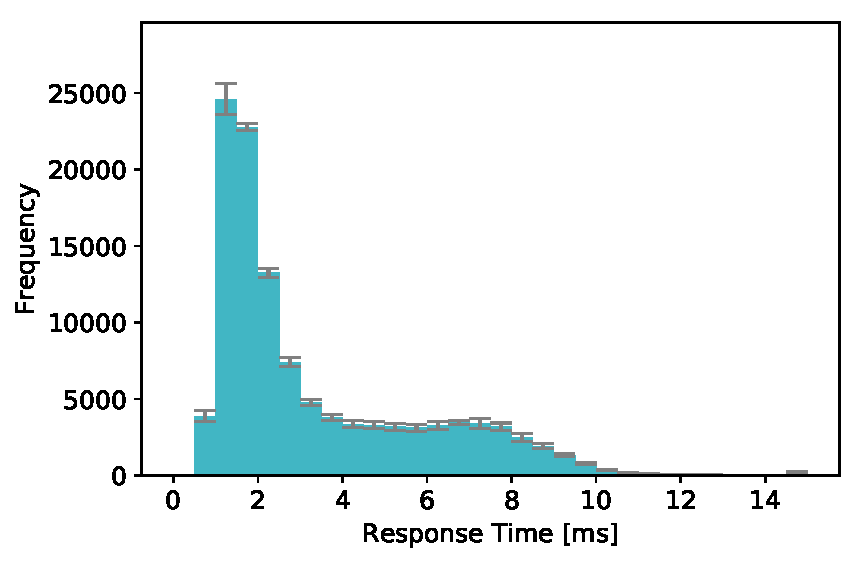
\includegraphics[width=\linewidth]{data/exp51_sharded_mget6_hist_mw.pdf}
		\caption{Sharded - Middleware}\label{fig1a}
	\end{subfigure}\hfill
	\begin{subfigure}[b]{.49\linewidth}
		\centering
		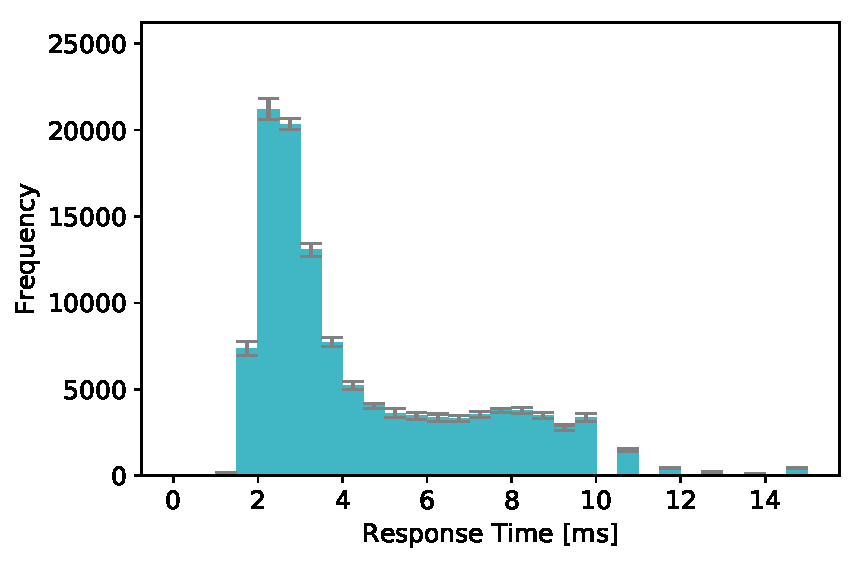
\includegraphics[width=\linewidth]{data/exp51_sharded_mget6_hist_client.pdf}
		\caption{Sharded - Client}\label{fig1b}
	\end{subfigure} \\
	\begin{subfigure}[b]{.49\linewidth}
		\centering
		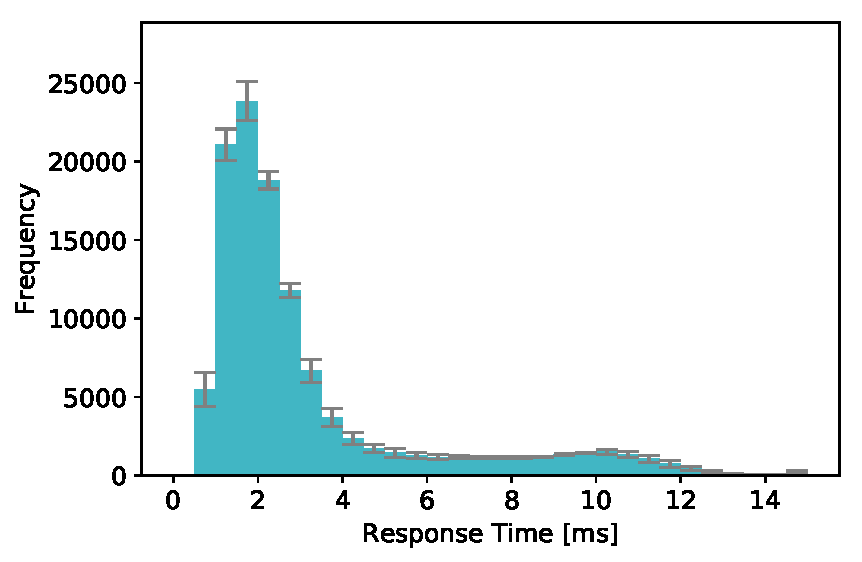
\includegraphics[width=\linewidth]{data/exp52_nonsharded_mget6_hist_mw.pdf}
		\caption{Non-Sharded - Middleware}\label{fig1a}
	\end{subfigure}\hfill
	\begin{subfigure}[b]{.49\linewidth}
		\centering
		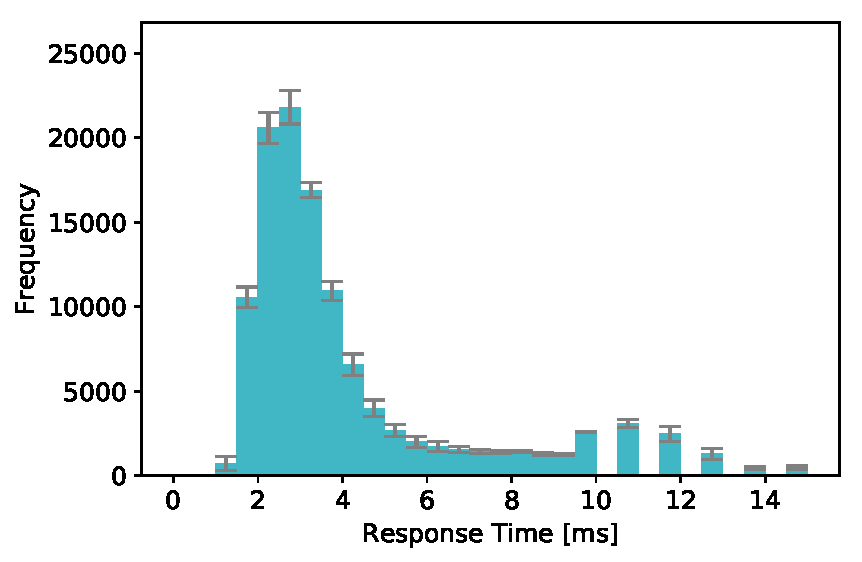
\includegraphics[width=\linewidth]{data/exp52_nonsharded_mget6_hist_client.pdf}
		\caption{Non-Sharded - Client}\label{fig1b}
	\end{subfigure}%
	\caption{Sharded and non-sharded response time distirbution for multi-gets with 6 keys as measured inside the middleware and on the client}
\end{figure}

\subsection{Summary}

Provide a detailed comparison of the sharded and non-shareded modes. For which multi-GET size is sharding the preferred option? Provide a detailed analysis of your system. Add any additional figures and experiments that help you illustrate your point and support your claims.

\section{2K Analysis (90 pts)}

For 3 client machines (with 64 total virtual clients per client VM) measure the throughput and response time of your system in a 2k experiment with repetitions. All GET operations have a single key. Investigate the following parameters:

\begin{itemize}
		
	\item Memcached servers: 1 and 3
	\item Middlewares: 1 and 2
	\item Worker threads per MW: 8 and 32
	      	      
\end{itemize}

Repeat the experiment for (a)~a write-only and (b)~a read-only workload.
For each of the two workloads, what is the impact of these parameters on throughput, respectively response time?

\begin{center}
	\scriptsize{
		\begin{tabular}{|l|c|}
			\hline Number of servers                & 1 and 3                                     \\ 
			\hline Number of client machines        & 3                                           \\ 
			\hline Instances of memtier per machine & 1 (1 middleware) or 2 (2 middlewares) \\ 
			\hline Threads per memtier instance     & 2 (1 middleware) or 1 (2 middlewares)   \\
			\hline Virtual clients per thread       &  32                                     \\ 
			\hline Workload                         & Write-only and Read-only\\
			\hline Multi-Get behavior               & N/A                                         \\
			\hline Multi-Get size                   & N/A                                         \\
			\hline Number of middlewares            & 1 and 2                                     \\
			\hline Worker threads per middleware    & 8 and 32                                    \\
			\hline Repetitions                      & 3 or more (at least 1 minute each)                                   \\ 
			\hline 
		\end{tabular}
	} 
\end{center}


\begin{table}
	\centering
	\small{
		\caption{$2^k3$ Experiment Base Table for Write-Only}
		\label{exp60_wo_2k_base} 
		\setlength{\tabcolsep}{4.5pt}
		\begin{tabular}{|c|rrrrrrrr|c|c|c|c|}
       \cline{10-13}
       \multicolumn{9}{c}{} & \multicolumn{2}{|c}{\textbf{Throughput} (ops/sec)} & \multicolumn{2}{|c|}{\textbf{Response Time} (ms)}\TBstrut\\
       \hline
       i & \hphantom{-}I\hphantom{-} & \hphantom{-}S\hphantom{-} & \hphantom{-}M\hphantom{-} &\hphantom{-}W\hphantom{-} & SM & SW & MW & SMW & ($y_{i1}, y_{i2}, y_{i3}$) & $\hat{y_i}$  & ($y_{i1}, y_{i2}, y_{i3}$) & $\hat{y_i}$\TBstrut\\
       \hline
   \Tstrut 1 & 1\hphantom{-} & -1\hphantom{-} & -1\hphantom{-} & -1\hphantom{--} & 1\hphantom{--} & 1\hphantom{--} & 1\hphantom{--} & -1\hphantom{---} & (6248, 6306, 6262) & 6272 & (28.6, 28.5, 28.7) & 28.6 \\
   2 & 1\hphantom{-} & 1\hphantom{-} & -1\hphantom{-} & -1\hphantom{--} & -1\hphantom{--} & -1\hphantom{--} & 1\hphantom{--} & 1\hphantom{---} & (5293, 5110, 5066) & 5157 & (33.8, 34.2, 35.5) & 34.5 \\
   3 & 1\hphantom{-} & -1\hphantom{-} & 1\hphantom{-} & -1\hphantom{--} & -1\hphantom{--} & 1\hphantom{--} & -1\hphantom{--} & 1\hphantom{---} & (8212, 8211, 8210) & 8211 & (21.4, 21.2, 21.2) & 21.3 \\
   4 & 1\hphantom{-} & 1\hphantom{-} & 1\hphantom{-} & -1\hphantom{--} & 1\hphantom{--} & -1\hphantom{--} & -1\hphantom{--} & -1\hphantom{---} & (6718, 6585, 6784) & 6696 & (25.7, 24.7, 25.9) & 25.4 \\
   5 & 1\hphantom{-} & -1\hphantom{-} & -1\hphantom{-} & 1\hphantom{--} & 1\hphantom{--} & -1\hphantom{--} & -1\hphantom{--} & 1\hphantom{---} & (9474, 9964, 9997) & 9812 & (16.0, 17.5, 17.4) & 17.0 \\
   6 & 1\hphantom{-} & 1\hphantom{-} & -1\hphantom{-} & 1\hphantom{--} & -1\hphantom{--} & 1\hphantom{--} & -1\hphantom{--} & -1\hphantom{---} & (7734, 7707, 7639) & 7693 & (22.2, 22.2, 22.4) & 22.3 \\
   7 & 1\hphantom{-} & -1\hphantom{-} & 1\hphantom{-} & 1\hphantom{--} & -1\hphantom{--} & -1\hphantom{--} & 1\hphantom{--} & -1\hphantom{---} & (12300, 12250, 11909) & 12153 & (13.7, 13.8, 13.1) & 13.5 \\
   8 & 1\hphantom{-} & 1\hphantom{-} & 1\hphantom{-} & 1\hphantom{--} & 1\hphantom{--} & 1\hphantom{--} & 1\hphantom{--} & 1\hphantom{---} & (9208, 9864, 9589) & 9554 & (16.4, 17.1, 16.0) & 16.5 \\
   \hline
    \end{tabular}
	}
\end{table}


\begin{table}
	\small{
		\centering
		\caption{Write-Only}
		\label{exp60_wo_2k_effect}
		\setlength{\tabcolsep}{4.7pt}
		\newcommand{\rlft}[0]{\raggedleft\arraybackslash}
		\begin{tabular}
       {|p{9mm}|% Factor
       p{8mm}% Tp Effect
       p{12mm}% Tp SS
       p{18.5mm}% Tp Variation
       p{22mm}|% Tp CI
       p{8mm}% Rt Effect
       p{12mm}% Rt SS
       p{18.5mm}% Rt Variation
       p{22mm}|} % Rt CI
       \cline{2-9}
       \multicolumn{1}{c}{} & \multicolumn{4}{|c}{\textbf{Throughput} (ops/sec)} & \multicolumn{4}{|c|}{\textbf{Response Time} (ms)}\TBstrut \\
       \hline
       \TBstrut Factor & Effect & Sum of\newline Squares & Percentage\newline of Variation & Confidence\newline Interval 90\% & Effect & Sum of\newline Squares & Percentage\newline of Variation & Confidence\newline Interval 90\%\\
       \hline
\Tstrut   I & $8193$\rlft & $1611160$k\rlft & $ $\rlft & $(8128,8259)^{\hphantom{a}}$\rlft & $22.4$\rlft & $12027$\rlft & $ $\rlft & $(22.2,22.6)^{\hphantom{a}}$\rlft \\   S & $-919$\rlft & $20250$k\rlft & $18.9$\rlft & $(-984,-853)^{\hphantom{a}}$\rlft & $2.3$\rlft & $125$\rlft & $12.3$\rlft & $(2.1,2.5)^{\hphantom{a}}$\rlft \\   M & $960$\rlft & $22116$k\rlft & $20.6$\rlft & $(895,1025)^{\hphantom{a}}$\rlft & $-3.2$\rlft & $247$\rlft & $24.2$\rlft & $(-3.4,-3.0)^{\hphantom{a}}$\rlft \\   W & $1610$\rlft & $62181$k\rlft & $58.0$\rlft & $(1544,1675)^{\hphantom{a}}$\rlft & $-5.1$\rlft & $617$\rlft & $60.4$\rlft & $(-5.3,-4.9)^{\hphantom{a}}$\rlft \\   SM & $-110$\rlft & $291$k\rlft & $0.3$\rlft & $(-175,-45)^{\hphantom{a}}$\rlft & $-0.5$\rlft & $6$\rlft & $0.6$\rlft & $(-0.7,-0.3)^{\hphantom{a}}$\rlft \\   SW & $-261$\rlft & $1633$k\rlft & $1.5$\rlft & $(-326,-196)^{\hphantom{a}}$\rlft & $-0.2$\rlft & $1$\rlft & $0.1$\rlft & $(-0.4,-0.0)^{\hphantom{a}}$\rlft \\   MW & $91$\rlft & $197$k\rlft & $0.2$\rlft & $(25,156)^{\hphantom{a}}$\rlft & $0.9$\rlft & $19$\rlft & $1.9$\rlft & $(0.7,1.1)^{\hphantom{a}}$\rlft \\   SMW & $-10$\rlft & $2$k\rlft & $0.0$\rlft & $(-75,55)^{a}$\rlft & $-0.1$\rlft & $0$\rlft & $0.0$\rlft & $(-0.3,0.1)^{a}$\rlft \\Error & & $535k$\rlft & $0.5$\rlft & & & $5.0$\rlft & $0.5$\rlft &\\   \hline
    \end{tabular}
	}
\end{table}



\begin{table}
	\centering
	\small{
		\caption{$2^k3$ Experiment Base Table for Read-Only}
		\label{exp60_ro_2k_base} 
		\setlength{\tabcolsep}{4.5pt}
		\begin{tabular}{|c|rrrrrrrr|c|c|c|c|}
       \cline{10-13}
       \multicolumn{9}{c}{} & \multicolumn{2}{|c}{\textbf{Throughput} (ops/sec)} & \multicolumn{2}{|c|}{\textbf{Response Time} (ms)}\TBstrut\\
       \hline
       i & \hphantom{-}I\hphantom{-} & \hphantom{-}S\hphantom{-} & \hphantom{-}M\hphantom{-} &\hphantom{-}W\hphantom{-} & SM & SW & MW & SMW & ($y_{i1}, y_{i2}, y_{i3}$) & $\hat{y_i}$  & ($y_{i1}, y_{i2}, y_{i3}$) & $\hat{y_i}$\TBstrut\\
       \hline
   \Tstrut 1 & 1\hphantom{-} & -1\hphantom{-} & -1\hphantom{-} & -1\hphantom{--} & 1\hphantom{--} & 1\hphantom{--} & 1\hphantom{--} & -1\hphantom{---} & (2890, 2895, 2898) & 2894 & (63.0, 63.1, 63.0) & 63.1 \\
   2 & 1\hphantom{-} & 1\hphantom{-} & -1\hphantom{-} & -1\hphantom{--} & -1\hphantom{--} & -1\hphantom{--} & 1\hphantom{--} & 1\hphantom{---} & (7779, 8234, 8203) & 8072 & (21.6, 21.5, 21.6) & 21.6 \\
   3 & 1\hphantom{-} & -1\hphantom{-} & 1\hphantom{-} & -1\hphantom{--} & -1\hphantom{--} & 1\hphantom{--} & -1\hphantom{--} & 1\hphantom{---} & (2879, 2790, 2879) & 2849 & (62.3, 60.1, 62.6) & 61.7 \\
   4 & 1\hphantom{-} & 1\hphantom{-} & 1\hphantom{-} & -1\hphantom{--} & 1\hphantom{--} & -1\hphantom{--} & -1\hphantom{--} & -1\hphantom{---} & (8339, 8610, 8481) & 8477 & (18.5, 20.1, 19.7) & 19.5 \\
   5 & 1\hphantom{-} & -1\hphantom{-} & -1\hphantom{-} & 1\hphantom{--} & 1\hphantom{--} & -1\hphantom{--} & -1\hphantom{--} & 1\hphantom{---} & (2903, 2905, 2896) & 2902 & (62.8, 61.8, 62.7) & 62.4 \\
   6 & 1\hphantom{-} & 1\hphantom{-} & -1\hphantom{-} & 1\hphantom{--} & -1\hphantom{--} & 1\hphantom{--} & -1\hphantom{--} & -1\hphantom{---} & (8693, 8686, 8693) & 8690 & (20.1, 19.6, 20.1) & 19.9 \\
   7 & 1\hphantom{-} & -1\hphantom{-} & 1\hphantom{-} & 1\hphantom{--} & -1\hphantom{--} & -1\hphantom{--} & 1\hphantom{--} & -1\hphantom{---} & (2885, 2877, 2868) & 2877 & (62.1, 61.6, 61.7) & 61.8 \\
   8 & 1\hphantom{-} & 1\hphantom{-} & 1\hphantom{-} & 1\hphantom{--} & 1\hphantom{--} & 1\hphantom{--} & 1\hphantom{--} & 1\hphantom{---} & (8635, 8621, 8613) & 8623 & (18.8, 19.1, 19.8) & 19.2 \\
   \hline
    \end{tabular}
	}
\end{table}


\begin{table}
	\small{
		\centering
		\caption{Read-Only}
		\label{exp60_ro_2k_effect}
		\setlength{\tabcolsep}{4.7pt}
		\newcommand{\rlft}[0]{\raggedleft\arraybackslash}
		\begin{tabular}
       {|p{9mm}|% Factor
       p{7.8mm}% Tp Effect
       p{12.6mm}% Tp SS
       p{17.9mm}% Tp Variation
       p{21.8mm}|% Tp CI
       p{7.8mm}% Rt Effect
       p{11.5mm}% Rt SS
       p{17.9mm}% Rt Variation
       p{24mm}|} % Rt CI
       \cline{2-9}
       \multicolumn{1}{c}{} & \multicolumn{4}{|c}{\textbf{Throughput} (ops/sec)} & \multicolumn{4}{|c|}{\textbf{Response Time} (ms)}\TBstrut \\
       \hline
       \TBstrut Factor & Effect & Sum of\newline Squares & Percentage\newline of Variation & Confidence\newline Interval 90\% & Effect & Sum of\newline Squares & Percentage\newline of Variation & Confidence\newline Interval 90\%\\
       \hline
\Tstrut   I & $5638$\rlft & $762787$k\rlft & $ $\rlft & $(5626,5650)^{\hphantom{a}}$\rlft & $42.9$\rlft & $44204$\rlft & $ $\rlft & $(42.8,43.1)^{\hphantom{a}}$\rlft \\   S & $2692$\rlft & $173961$k\rlft & $95.5$\rlft & $(2680,2704)^{\hphantom{a}}$\rlft & $-20.9$\rlft & $10439$\rlft & $99.1$\rlft & $(-21.0,-20.7)^{\hphantom{a}}$\rlft \\   M & $238$\rlft & $1363$k\rlft & $0.7$\rlft & $(226,250)^{\hphantom{a}}$\rlft & $-0.9$\rlft & $19$\rlft & $0.2$\rlft & $(-1.0,-0.7)^{\hphantom{a}}$\rlft \\   W & $239$\rlft & $1371$k\rlft & $0.8$\rlft & $(227,251)^{\hphantom{a}}$\rlft & $-0.8$\rlft & $17$\rlft & $0.2$\rlft & $(-1.0,-0.7)^{\hphantom{a}}$\rlft \\   SM & $235$\rlft & $1330$k\rlft & $0.7$\rlft & $(223,248)^{\hphantom{a}}$\rlft & $-0.7$\rlft & $10$\rlft & $0.1$\rlft & $(-0.8,-0.5)^{\hphantom{a}}$\rlft \\   SW & $237$\rlft & $1353$k\rlft & $0.7$\rlft & $(225,250)^{\hphantom{a}}$\rlft & $-0.8$\rlft & $15$\rlft & $0.1$\rlft & $(-1.0,-0.6)^{\hphantom{a}}$\rlft \\   MW & $-239$\rlft & $1367$k\rlft & $0.8$\rlft & $(-251,-227)^{\hphantom{a}}$\rlft & $0.8$\rlft & $16$\rlft & $0.2$\rlft & $(0.7,1.0)^{\hphantom{a}}$\rlft \\   SMW & $-239$\rlft & $1374$k\rlft & $0.8$\rlft & $(-251,-227)^{\hphantom{a}}$\rlft & $0.7$\rlft & $11$\rlft & $0.1$\rlft & $(0.5,0.8)^{\hphantom{a}}$\rlft \\Error & & $18k$\rlft & $0.0$\rlft & & & $3.0$\rlft & $0.0$\rlft &\\   \hline
    \end{tabular}
	}
\end{table}

\section{Queuing Model (90 pts)}

Note that for queuing models it is enough to use the experimental results from the previous sections. It is, however, possible that the numbers you need are not only the ones in the figures we asked for, but also the internal measurements that you have obtained through instrumentation of your middleware.

\subsection{M/M/1}

Build queuing model based on Section 4 (write-only throughput) for each worker-thread configuration of the middleware. Use one M/M/1 queue to model your entire system. Motivate your choice of input parameters to the model. Explain for which experiments the predictions of the model match and for which they do not.

\subsection{M/M/m}

Build an M/M/m model based on Section 4, where each middleware worker thread is represented as one service.  Motivate your choice of input parameters to the model. Explain for which experiments the predictions of the model match and for which they do not.

\subsection{Network of Queues}

Based on Section 3, build a network of queues which simulates your system. Motivate the design of your network of queues and relate it wherever possible to a component of your system. Motivate your choice of input parameters for the different queues inside the network. Perform a detailed analysis of the utilization of each component and clearly state what the bottleneck of your system is. Explain for which experiments the predictions of the model match and for which they do not.


\bibliography{bibdb}{}
\bibliographystyle{plain}
\end{document}
